\documentclass[a4paper, 12pt]{report}
\usepackage[latin1]{inputenc}
\usepackage[italian]{babel}
\usepackage[T1]{fontenc}
\usepackage{graphicx}
\usepackage{float}
\usepackage[centertags]{amsmath}
\usepackage{amsfonts}
\usepackage{amssymb}
\usepackage{amsthm}
\usepackage{newlfont}
\usepackage{fancyhdr}
\usepackage{tesisty}
\usepackage{quoting}
\usepackage{url} 
\usepackage{listings}
\usepackage{epstopdf}
\usepackage{color}

\definecolor{javared}{rgb}{0.6,0,0} % for strings
\definecolor{javagreen}{rgb}{0.25,0.5,0.35} % comments
\definecolor{javapurple}{rgb}{0.5,0,0.35} % keywords
\definecolor{javadocblue}{rgb}{0.25,0.35,0.75} % javadoc

\lstset{language=Java,
	basicstyle=\small,
	keywordstyle=\color{javapurple}\bfseries,
	stringstyle=\color{javagreen},
	commentstyle=\color{javared},
	morecomment=[s][\color{javadocblue}]{/**}{*/},
	stepnumber=2,
	numbersep=10pt,
	tabsize=4,
	showspaces=false,
	showstringspaces=false}


\quotingsetup{font=small}

%-------------------------------
% DEFINIZIONE DEGLI ENVIRONMENT
%-------------------------------

\newtheorem{obs}{Osservazione}[section]
\newenvironment{oss}
    {\begin{obs}\begin{normalfont}}
    {\hfill $\square \!\!\!\!\checkmark$ \end{normalfont}\end{obs}}

\newtheorem{pro}{Problema}[chapter]
\newenvironment{prob}
    {\begin{pro}\begin{normalfont}}
    {\hfill $\spadesuit$ \end{normalfont}\end{pro}}

\newtheorem{teor}{Teorema}[section]
\newenvironment{teorema}
    {\begin{teor}\textit }
    {\hfill  \end{teor}}

\newtheorem{defn}{Definizione}[section]
\newenvironment{de}
    {\begin{defn}\begin{normalfont}}
    {\hfill $\clubsuit$ \end{normalfont}\end{defn}}

%-----------------------------
% CONFIGURAZIONE DELLA PAGINA
%-----------------------------

\hfuzz2pt % Don't bother to report over-full boxes if over-edge is < 2pt

\fancypagestyle{plain}{
\fancyhead{}\renewcommand{\headrulewidth}{0pt} } \pagestyle{fancy}
\renewcommand{\chaptermark}[1]{\markboth{\small CAP. \thechapter \textit{ #1}} {} }
\renewcommand{\sectionmark}[1]{\markright{\small  \thesection \textit{ #1}} {} }
\voffset=-20pt    % distanza tra il limite superiore del foglio e l'intestazione
\headsep=40pt     % distanza  l'intestazione ed il testo del corpo
\hoffset=0 pt     % misura equivalente al margine sinistro
\textheight=620pt % altezza del corpo del testo
\textwidth=435pt  % larghezza del corpo del testo
\footskip=40pt    % distanza tra il testo del corpo ed il pie' di pagina
\fancyhead{}      % cancella qualsiasi impostazione per l'intestazione
\fancyfoot{}      % cancella qualsiasi impostazione per il pie' di pagina
\headwidth=435pt  % larghezza del'intestazione e del pie' di pagina
\fancyhead[R]{\rightmark} \fancyfoot[L]{\leftmark}
\fancyfoot[R]{\thepage}
\renewcommand{\headrulewidth}{0.3pt}   % spessore della linea dell'intestazione
\renewcommand{\footrulewidth}{0.3pt}   % spessore della linea del pi�di pagina

\numberwithin{equation}{section}
\renewcommand{\theequation}{\thesection.\arabic{equation}}


%--------------------------
% MODIFICARE DA QUI IN POI
%--------------------------

\begin{document}
\begin{center}
%
\includegraphics[width=0.1\linewidth]{./imgs/icon}
\end{center}

%\dedicate{A coloro il cui supporto non verrà mai dimenticato}
\begin{center}
\corso{Sicurezza Informatica e Internet} 
\titoloTesi{Build Your Own Botnet v.1} \anno{2015/2016}
\end{center}
\autore{0211577 - Cappello Domenico - domenico.cappello@gmail.com\\
0213347 - Nazio Alessio - alessio.nazio@gmail.com}

\baselineskip=25pt

\intestazione

%------------------------------------------------
% INTRODUZIONE E RINGRAZIAMENTI (NON MODIFICARE)
%------------------------------------------------

\fancypagestyle{plain}{
\fancyhead{}\renewcommand{\headrulewidth}{0pt} } \pagestyle{fancy}
\renewcommand{\chaptermark}[1]{\markboth{\small Cap. \thechapter \textit{ #1}} {} }
\renewcommand{\sectionmark}[1]{\markright{\small  \S \thesection \textit{ #1}} {} }
\voffset=-20pt                         % distanza tra il limite superiore del foglio e l'intestazione
\headsep=40pt                          % distanza  l'intestazione ed il testo del corpo
\hoffset=0pt                           % misura equivalente al margine sinistro
\textheight=620pt                      % altezza del corpo del testo
\textwidth=435pt                       % larghezza del corpo del testo
\footskip=40pt                         % distanza tra il testo del corpo ed il pie' di pagina
\fancyhead{}                           % cancella qualsiasi impostazione per l'intestazione
\fancyfoot{}                           % cancella qualsiasi impostazione per il pie' di pagina
\headwidth=435pt                       % larghezza del'intestazione e del pie' di pagina
\fancyhead[R]{\rightmark} \fancyfoot[L]{\leftmark}
\fancyfoot[R]{\thepage}
\renewcommand{\headrulewidth}{0.3pt}   % spessore della linea dell'intestazione
\renewcommand{\footrulewidth}{0.3pt}   % spessore della linea del pi�di pagina

\pagenumbering{Roman} \tableofcontents
\newpage

\pagenumbering{arabic}

%\fancyhead[R]{Abstract} \fancyfoot[L]{}
%\fancyfoot[R]{\thepage}
%\include{Abstract}

\fancyhead[R]{Introduzione} \fancyfoot[L]{}
\fancyfoot[R]{\thepage}
\chapter{Introduzione}
\section{Premessa}
Oggigiorno, la maggior parte dei PC utilizza sistemi operativi senza patch e/o senza alcuna sicurezza dietro un \textit{firewall}, rendendoli facili prede di attacchi diretti, orchestrati da malintenzionati, e di attacchi di tipo indiretto, mascherati dietro programmi che l'utente utilizza costantemente (vedi reti \textit{P2P}).\\
Con l'incremento delle connessioni a banda larga si ha avuto anche un incremento del numero di potenziali vittime di attacchi, con cui i malintenzionati traggono beneficio dalla situazione, utilizzandola a loro vantaggio, sfruttando anche l'automatizzazione di tecniche per la scansione di porzioni della rete che semplifica la ricerca di sistemi vulnerabili. Una volta che un vasto numero di macchine sono state infettate, esse entrano a far parte di una ``rete di macchine compromesse che posso essere controllate da remoto\footnote{Provos Niels, Holz Thorsten (2007).}'', chiamata \textbf{botnet}.\\
Una \textit{botnet} consiste di tre elementi principali che sono i bot (cio\`e le macchine infettate che ne fanno parte), il \textit{command and control server} (C\&C - da cui ogni bot riceve istruzioni e con cui il malintenzionato ha privilegi amministrativi remoti su tutte le macchine infette) ed il \textit{botmaster}; si basa, inoltre, su quattro concetti chiave:
\begin{enumerate}
\item le \textit{botnet} sono reti, quindi sistemi in cui la comunicazione \`e importante;
\item le macchine che fanno parte di una \textit{botnet} sono, tipicamente, partecipanti ignari;
\item i \textit{bot} sono controllabili da remoto, permettendo di fare rapporto o ricevere ordini da una struttura C\&C (centralizzata o decentralizzata);
\item i \textit{bot} sono controllati da persone con intenti malevoli che fanno capo a qualche forma di attivit\`{a} illegale.
\end{enumerate}

\vspace*{1cm}
\section{HTTP Botnet}
\begin{figure}[h]
        \centering
		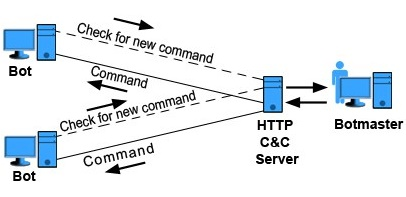
\includegraphics[width=0.5\linewidth]{./imgs/botnet1999}
        \caption{Struttura di una botnet}
        \label{strutturabotnet}
\end{figure}
Quando il protocollo HTTP nacque nel 1999, nessuno avrebbe mai pensato che sarebbe stato utilizzato per le botnet. 
La prima generazione di botnet utilizzava l'\textit{Internet Relay Chat} (IRC\footnote{Protocollo di messaggistica istantanea su Internet, che consente sia la comunicazione diretta fra due utenti, che il dialogo contemporaneo di gruppi di persone raggruppati in stanze di discussione dette canali.}) e relativi canali per instaurare un meccanismo di ``controllo e comando''. I bot IRC seguono lo stesso approccio PUSH di quando ci si unisce ai canali, rimanendo connessi. Essi si connettono ai server IRC e ai canali che sono stati selezionati dal \textit{botmaster} e attendono comandi. 
Invece di rimanere connessi, i bot HTTP controllano periodicamente per aggiornamenti oppure nuovi comandi: questo modello \`e detto di PULL e continua ad intervalli regolari definiti dal botmaster, che usa il protocollo HTTP per nascondere le proprie attivit\`{a} tra il normale flusso web, riuscendo ad evitare facilmente i metodi di rivelazione come i \textit{firewall}. 

\vspace*{1cm}
\section{Obiettivo}
L'obiettivo \`e quello di sviluppare un software per workstation che definisca bot in grado di contattare delle URL a cui sono associati una serie di parametri fondamentali:
\begin{enumerate}
\item la periodicit\`{a} di contatto (fissa o variabile in un intervallo temporale);
\item il numero massimo di contatti da effettuare;
\item una eventuale modalit\`{a} di ``\textit{sleep}'', intesa come insieme di condizioni in cui non viene effettuata nessuna azione ;
\item un eventuale user-agent ``\textit{custom}'';
\item l'indirizzo ip e la porta di un eventuale ``\textit{proxy}'' pubblico.
\end{enumerate}
Tali parametri saranno impostati tramite un file di testo (pre-compilato oppure configurabile mediante una \textit{Graphic User Interface}).\\
I contatti effettuati e i parametri di configurazione in uso verranno salvati su un file di log;
le informazioni principali relative alla macchina su cui il codice \`{e} in esecuzione saranno salvate nel file \textit{sys\_info.txt}.

%\vspace*{1cm}
%\section{Struttura della relazione}
%L'analisi, la progettazione e  sviluppo del progetto inizia con un'esposizione del programma implementato, spiegandone la logica, ed esponendo il tentativo di conferire una modalit\'a di utilizzo immediata, con poche piccole azioni. Nel capitolo successivo si parler\'a degli elementi principali del progetto e tutto ci\`o che li riguarda, evidenziandone il processo di analisi. A seguire, un capitolo dedicato alle metodologie utilizzate per la creazione dei bot facenti parti della rete. Infine, l'ultimo punto, \`e quello dell'analisi dei casi di test effettuati per un corretto funzionamento del programma.

\fancyhf{} %elimina header/footer vecchi


\fancyhead[R]{\rightmark} \fancyhead[L]{\leftmark}
\fancyfoot[R]{\thepage}





%---------------------
% INCLUSIONE CAPITOLI
%---------------------

\chapter{Panoramica del progetto}
\begin{minipage}{12cm}\textit{Nel capitolo verr\`{a} effettuata una breve introduzione alle componenti principali del progetto, verr\`{a} esposto il percorso di progettazione seguito per un suo corretto sviluppo, e illustrato l'utilizzo del software da parte dell'utente.}
\end{minipage}

\vspace*{1cm}
\section{Componenti principali}
Le entit\`{a} principali presenti nel software realizzato sono un \textit{Parser}, con il ruolo di interpretare le informazioni contenute nel file di configurazione, uno \textit{Scheduler}, che ha il compito di garantire la corretta esecuzione dei task al termine delle rispettive scadenze, un protocollo di comunicazione (\textit{HTTP}) con cui interrogare le macchine specificate. Nello sviluppo dell'applicativo \textit{multi-piattaforma} \`{e} stato utilizzato il \textit{Singleton pattern}, per evitare la creazione di istanze multiple dello scheduler o del logger.
In ottica di una futura integrazione del software in una rete di bot, sono state inserite funzioni per il calcolo di un ID univoco per ogni macchina appartenente alla rete controllata.

\vspace*{0.5cm}
\subsection{HTTP}
\textbf{HTTP}, acronimo di \textit{hypertext transfer protocol}.
\`E un protocollo a livello applicativo utilizzato per la
trasmissione di informazioni tramite un meccanismo di richiesta/risposta tra \textit{client} e \textit{server}. All'interno del messaggio di richiesta sono definiti diversi campi tra cui il tipo di
richiesta (\textit{GET}, \textit{POST}) e lo \textit{UserAgent}, che identifica la tipologia di \textit{client} utilizzata.
Il metodo \textit{GET} pu\`{o} essere utilizzato per effettuare una richiesta:
\begin{itemize}
	\item \textbf{assoluta}, senza ulteriori specificazioni sulla risorsa cercata;
	\item \textbf{condizionale}, se nell'\textit{header} del messaggio di richiesta sono presenti i campi \textit{If-Modified-Since}, \textit{If-Match}, etc.;
	\item \textbf{parziale}, quando la risorsa richiesta \`e una sottoparte di una risorsa memorizzata.
\end{itemize}
Nel software sono effettuate solo \textit{GET} assolute, e la scelta dello \textit{user-agent} \`{e} lasciata alla discrezione dell'utilizatore.

\vspace*{0.5cm}
\subsection{Singleton Pattern}
In determinati contesti \`e necessario che venga istanziato un solo esemplare di una classe. Ad esempio: per evitare due riproduzioni audio contemporanee, sar\`{a} opportuno istanziare un riproduttore musicale una sola volta,
uno \textit{spooler} di stampa dovrebbe tenere una coda unica anche se sono presenti pi\`{u} stampanti attive e
il manager di un file system dovrebbe essere unico.

Per garantire questa singola istanziazione \`{e} sufficiente rendere impossible l'utilizzo del costruttore della classe da parte del resto del codice, e fornire un metodo indiretto per ottenere una istanza (l'unica) di tale classe.
Sono quindi possibili diverse soluzioni:
\begin{itemize}
	\item dichiarare privato il costruttore, in modo che esso possa essere visto solo all'interno della classe Singleton;
	\item prevedere il metodo (pubblico) statico e cio\`e di classe, in modo che esso sia comunque visibile. Questo metodo deve istanziare un esemplare se ci\`o non \`e ancora accaduto, oppure restituire l'oggetto gi\'a istanziato in precedenza senza istanziare ulteriori esemplari.
\end{itemize}
Questa seconda scelta \`e quella applicata nel progetto per la creazione e gestione del \textit{logger} e la creazione di uno schedulatore di task.

\vspace*{0.5cm}
\subsection{Scheduler}
Lo \textit{scheduler} ha il compito di garantire la corretta esecuzione dei task al termine delle rispettive scadenze.

Nell'applicativo \`{e} stato utilizzato uno \textit{Scheduler Executor Service}, istanziato una sola volta mediante l'uso del \textit{Singleton pattern}; data la presenza di istruzioni bloccanti nei task da eseguire, \`{e} stato messo a disposizione dello scheduler un pool di $30$ \textit{thread}.

La classe utilizzata permette la schedulazione di job periodici tramite la funzione \textit{scheduleAtFixedRate} ma, data la necessit\`{a} di schedulare task con rate non fissato, \`{e} stato deciso di effettuare le singole ri-schedulazioni utilizzando, la pi\`{u} semplice, funzione \textit{schedule}.


\vspace*{0.5cm}
\subsection{ID dei bot e MD5}
In una rete reale, i \textit{bot} sono univocamente identificabili dal centro di comando e controllo:
l'attaccante ha interesse nel conoscere il numero di \textit{bot} attivi per effettuare un attacco ad una data; questa informazione inoltre risulta fondamentale, a livello economico, se egli decide di vendere o affittare la \textit{botnet} ad un acquirente esterno. 

Per garantire l'unicit\`{a} dell'identificativo di ogni bot, viene effettuato l'\textit{hash md5} delle informazioni riguardanti l'hardware della macchina e il sistema operativo in esecuzione.

\vspace*{0.5cm}
\subsection{Parsing}
La corretta interpretazione del file di configurazione \`{e} garantita dal \textit{Parser} che, mediante la conoscenza del protocollo utilizzato per l'organizzazione delle informazioni e la manipolazione di oggetti di tipo stringa, genera dal file l'\textit{ArryList} dei task in attesa di esecuzione. 

La classe \`{e} utilizzata anche per l'operazione di scrittura del file di configurazione a partire dai \textit{form} riempiti dall'utente nell'interfaccia principale dell'applicazione.

\vspace*{0.5cm}
\subsection{Multi-piattaforma}
Quando si parla di un programma multi-piattaforma si intende un programma in grado di funzionare correttamente su diversi sistemi operativi.\\
Sono stati gestite quindi le funzionalit\`{a} dipendenti dalla piattaforma su cui l'applicativo \`{e} in esecuzione (come la generazione dell' ID univoco del bot o l'individuazione dei browser installati), differenziandone il comportamento sulla base del sistema operativo presente sulla macchina.

\vspace*{0.5cm}
\section{Piattaforma di sviluppo, Swing, Awt}
NetBeans \`e un ambiente di sviluppo integrato (\textit{IDE} -  \textit{Integrated Development Environment}) multi-linguaggio, scelto dalla Oracle Corporation come \textit{IDE} ufficiale da contrapporre al pi\'u diffuso Eclipse.\\
NetBeans utilizza due componenti principali: la piattaforma, che comprende una serie di librerie per fornire gli elementi base dell'\textit{IDE} come presentazione dei dati e interfaccia utente, e l'\textit{IDE} vero e proprio, che permette di gestire il controllo e le funzionalit\'a offerte dalla piattaforma. NetBeans utilizza \textit{Abstract Window Toolkit} (\textit{AWT}), un insieme di API realizzate da Sun che permettono agli sviluppatori di modellare le interfacce grafiche delle finestre, pulsanti e altri elementi visuali. \textit{AWT} fornisce gli elementi grafici base che dipendono dalla piattaforma utilizzata, mentre per gli aspetti di alto livello come gestione di colori e interazione con l'utente \`e usata la libreria Swing.

\vspace*{1cm}
\section{Build your own botnet}
In questa sezione sono presentati la struttura del progetto ed i principali casi d'uso dell'applicativo realizzato.

\vspace*{0.5cm}
\subsection{Struttura del progetto}
Il progetto \`e composto da diverse classi:
\begin{itemize}
\item \textbf{ByobComm}, responsabile del protocollo di comunicazione;
\item \textbf{ByobSingleton}, tramite il quale \`{e} stato implementato il \textit{Singleton pattern};
\item \textbf{ByobTask}, rappresenta il singolo \textit{task} che deve essere schedulato;
\item \textbf{Byob\_v1}, la classe principale, da cui viene avviata la GUI;
\item \textbf{GUI}, responsabile di ci\`{o} che riguarda la creazione e gestione della \textit{Graphic User Interface} ;
\item \textbf{Parser}, responsabile della creazione di file, lettura e scrittura dei parametri di configurazione inseriti dall'utente;
\item \textbf{Tools}, contenente varie funzioni e metodi utili in diversi contesti;
\item \textbf{URLDetails}, contenente i dati (parametri di configurazione) del singolo \textit{contatto} da effettuare.
\end{itemize} 

\vspace*{0.5cm}
\subsection{ByobComm}
La classe \textit{ByobComm} gestisce la comunicazione HTTP.
Se presente, viene configurato il \textit{proxy} specificato nel file di configurazione; si specifica il tipo di metodo HTTP utilizzato (GET), la codifica dell'\textit{header} e lo \textit{user agent}.
Per la connessione si \`{e} utilizzata la classe \textit{HttpURLConnection}.

\vspace*{0.5cm}
\subsection{ByobSingleton}
Responsabile del \textit{Singleton pattern} utilizzato, contiene al suo interno il \textit{Logger} dell'applicazione, che trascrive:

\begin{itemize}
\item i contatti e i parametri di configurazione;
\item il \textit{timestamp} di contatto e il dettaglio delle URL contattate;
\item le informazioni relative al Sistema Operativo e ai browser presenti sulla postazione su cui il software \`e installato.
\end{itemize}
Oltre al \textit{Logger}, la classe comprende al suo interno lo \textit{scheduler} dei \textit{task} da eseguire.

\vspace*{0.5cm}
\subsection{ByobTask}
\textit{ByobTask} rappresenta il singolo task che lo \textit{Scheduler Executor Service} deve eseguire.
Essa implementa l'interfaccia \textit{Runnable}, ed ogni istanza della classe ri-schedula la propria esecuzione in accordo con le informazioni immagazzinate nel contatto \textit{URLDetails} a cui \`{e} associata.

\vspace*{0.5cm}
\subsection{GUI}

La classe \textit{GUI} rappresenta l'interfaccia grafica tramite la quale l'utilizzatore pu\`{o} fornire i parametri di configurazione dell'applicazione.
Le azioni principali che possono essere intraprese sono due:
\begin{enumerate}
\item l'apertura di un file di configurazione gi\`{a} compilato (\textbf{Figura \ref{fig:gui}});
\item la creazione di un nuovo file di configurazione.
\end{enumerate}

\begin{figure}[!htb]
	\centering
	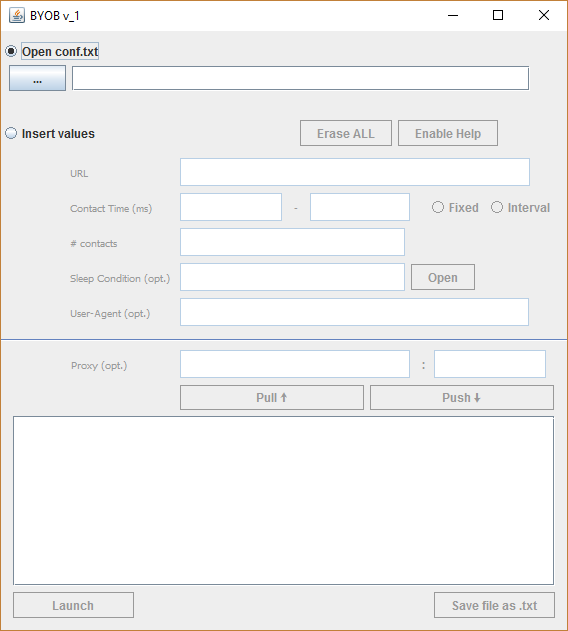
\includegraphics[width=0.7\linewidth]{./imgs/gui}
	\caption{Apertura di un file di configurazione}\label{fig:gui}
	\vspace*{0.5cm}
\end{figure}

\begin{figure}[!htb]
        \centering
		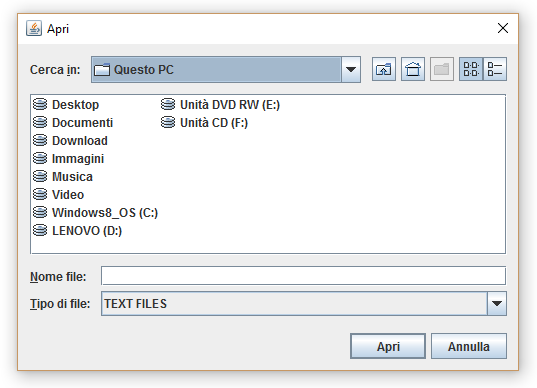
\includegraphics[width=0.6\linewidth]{./imgs/scelta1}
        \caption{JFileChooser}
        \label{fig:chooser}
\end{figure}

Alla pressione del tasto "...", un \textit{JFileChooser} permetter\`{a} la ricerca di un file di testo all'interno delle directory presenti nel dispositivo di memorizzazione in uso (\textbf{Figura \ref{fig:chooser}}).

\begin{figure}[!htb]
        \centering
		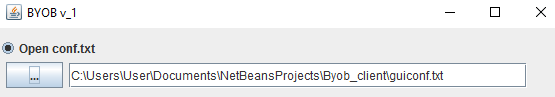
\includegraphics[width=0.7\linewidth]{./imgs/scelta11}
        \caption{Scelta del file di configurazione}
        \label{fig:conf}
\end{figure}

Una volta effettuata la selezione, il percorso assoluto del file scelto verr\`{a} scritto nella casella di testo relativa, e sar\`{a} attivato il tasto "Launch" per l'avvio dell'applicazione (\textbf{Figura \ref{fig:conf}}).

\begin{figure}[!htb]
        \centering        
        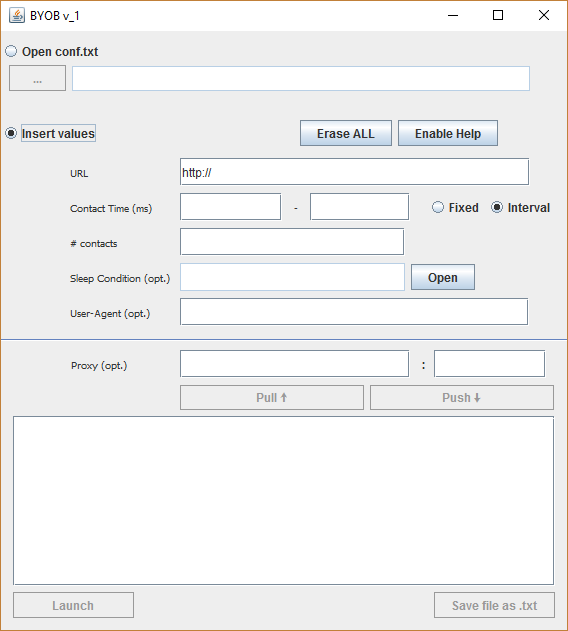
\includegraphics[width=0.7\linewidth]{./imgs/gui2}
        \caption{Inserimento manuale parametri di configurazione}
        \label{fig:manual}
\end{figure}

Tramite l'inserimento manuale dei parametri di configurazione, \`{e} possibile specificare (\textbf{Figura \ref{fig:manual}}):

\begin{itemize} 
\item la \textbf{URL} da contattare;
\item il \textbf{Contact Time}, ossia la periodicit\`{a} di contatto che pu\`{o} essere:
\begin{itemize}
\item [-] Fissa ("\textit{Fixed}");
\item [-] Invervallo ("\textit{Interval}"), cio\`e all'interno di un intervallo temporale;
\end{itemize} 
\item \textbf{\#contacts}, ossia il numero massimo di contatti da effettuare verso la URL specificata;
\item le \textbf{Sleep conditions} (campo opzionale), ovvero l'insieme delle condizioni temporali sotto le quali non deve essere svolta alcuna azione; 
\begin{figure}[!htb]
        \centering
		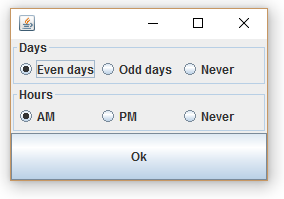
\includegraphics[width=0.4\linewidth]{./imgs/sleep}
        \caption{Sleep conditions}
\end{figure}
\begin{itemize}
\item [-] Condizione sui giorni pari (E), sui giorni dispari (O), nessuna restrizione;
\item [-] Condizione sulle prime dodici ore (A), condizione sulle ultime 12 ore (P), nessuna restrizione;
\end{itemize}
\item lo \textbf{User-Agent} (opzionale), ossia la modifica da apportare al campo User-Agent dell'header HTTP;
\item il \textbf{Proxy} (opzionale), ossia l'indirizzo IP e la porta di un proxy pubblico da utilizzare.
\end{itemize} 

Una volta inseriti nelle relative caselle di testo, il tasto "\textit{Push}" permette di visualizzare tali parametri nell' area sottostante (\textbf{Figura \ref{fig:push}}). 

Il tasto "\textit{Pull}" permette di estrarre dall'area di testo l'ultimo inserimento effettuato per una eventuale modifica dei parametri non correttamente inseriti.
\begin{figure}[!htb]
        \centering
		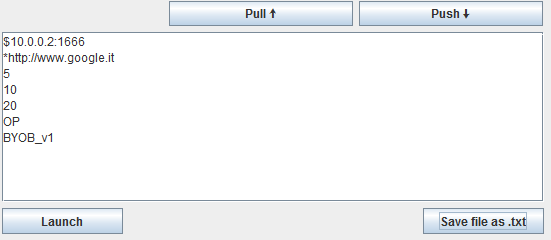
\includegraphics[width=0.6\linewidth]{./imgs/textarea}
        \caption{Push - Inserimento dell'input nell'area di testo}
        \label{fig:push}
        \vspace*{0.5cm}
\end{figure}

Al termine dell'inserimento manuale, la pressione del tasto "Save file as .txt" permette il salvataggio, tramite procedura guidata, del file di configurazione appena creato.

\paragraph{GUI user-friendly}
La pressione del tasto "Enable Help" permette la comparsa (al passaggio del mouse) di \textit{tooltip} sulle caselle del form, rendendone pi\`{u} immediata la corretta compilazione (\textbf{Figura \ref{fig:help}}).

\begin{figure}[!htb]
        \centering        
        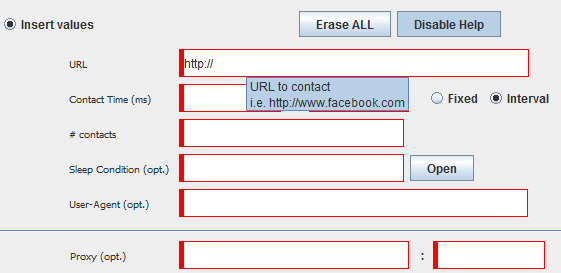
\includegraphics[width=0.7\linewidth]{./imgs/help}
        \caption{Utilizzo dell'help}
        \label{fig:help}
\end{figure}

La pressione del tasto "Erase ALL", da utilizzare in caso di molteplici errori, causa la cancellazione di tutto il file di configurazione compilato.

Nel caso vengano riscontrati degli errori al momento della pressione del tasto "Push", un popup guider\`{a} l'utilizzatore nella risoluzione dei problemi individuati (\textbf{Figura \ref{fig:warning}}).

\begin{figure}[!htb]
        \centering        
        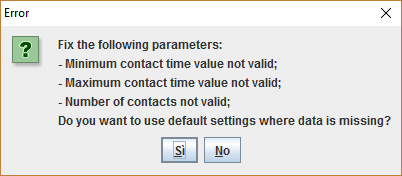
\includegraphics[width=0.6\linewidth]{./imgs/warning}
        \caption{Esempio di messaggio d'errore per dati mancanti e/o errati}
        \label{fig:warning}
\end{figure}

\vspace*{0.5cm}
\subsection{Parser}
La classe \textit{Parser} \`{e} responsabile di:
\begin{itemize}
\item lettura e scrittura del file contenente i parametri di configurazione;
\item creazione di una lista di istanze della classe \textit{URLDetails}, una per ciascun contatto da effettuare;
\item conversione dei parametri di configurazione;
\item controllo di validit\`{a} per ciascun parametro di configurazione.
\end{itemize}

\vspace*{0.5cm}
\subsection{Tools}
La classe \textit{Tools} contiene al suo interno diversi metodi statici, utili in pi\`{u} sezioni del programma.
Essa \`{e} responsabile della generazione dell'ID del bot, della prima schedulazione dei task programmati, della raccolta delle informazioni relative al sistema operativo e ai browser installati sulla macchina, dei controlli per la generazione dei \textit{warning messages} della classe GUI.

\vspace*{0.5cm}
\subsection{URLDetails}
\textit{URLDetails} \`e la classe che contiene le informazioni inserite dall'utente per ciascun contatto che deve essere effettuato.
\chapter{Implementazione}
\label{chap:implementazione}
\begin{minipage}{12cm}\textit{Sono di seguito presentati dettagli riguardanti l'implementazione dei passi principali eseguiti dal programma in esame. }
\end{minipage}

\section{Avvio iniziale}
All'avvio dell'applicazione, viene visualizzata la schermata principale di configurazione; vengono inoltre raccolte e scritte sul file \textit{sys\_info.txt} informazioni riguardanti il sistema operativo della macchina e le versioni dei browser installati.

\vspace{0.5cm}
\begin{lstlisting}
public class Byob_v1 {

	public static void main(String[] args) {
		/**Start the GUI*/
		GUI frame = new GUI();
		final Toolkit toolkit = Toolkit.getDefaultToolkit();
		final Dimension screenSize = toolkit.getScreenSize();
		int x = (screenSize.width - frame.getWidth()) / 2;
		int y = (screenSize.height - frame.getHeight()) / 2;
		frame.setTitle("BYOB v_1");
		frame.setLocation(x, y);
		frame.setVisible(true);
		/**Gather system informations and write them on sys_info.txt*/
		Tools.writeInfoFile("sys_info.txt");
	}

}
\end{lstlisting}

\section{Informazioni di sistema}

Il sistema operativo in esecuzione sulla macchina \`{e} restituito dalla funzione \textit{Tools.getOs()}.

\vspace{0.5cm}
\begin{lstlisting}
    public static String getOs(){
	    return System.getProperty("os.name");
    }
\end{lstlisting}

Per riuscire ad identificare i browser installati, sono state adottate strategie differenti per ogni sistema operativo individuato;
la funzione \textit{Tools.getBrowsers()} invoca \textit{Tools.getOs()} e distingue le azioni da intraprendere:

\vspace{0.5cm}
\begin{lstlisting}
public static String getBrowsers(){

	String browsers = "";
	String os = getOs().toLowerCase();
	if(os.contains("linux")){
		[...]
	} else if(os.contains("windows")){
		[...]
	} else if(os.contains("mac")){
		[...]
	} else {
		/**Couldn't recognize OS*/
	}
	return browsers;
\end{lstlisting}

\subsection{Linux}
I browser ritenuti pi\`{u} comuni in ambiente linux sono stati:
\begin{itemize}
	\item Google Chrome
	\item Mozilla Firefox
	\item Opera
	\item Chromium
\end{itemize}
Per identificare l'eventuale versione installata di ogni browser, viene avviato un nuovo processo che esegue la \textit{bash} invocando il programma relativo ad ogni browser con il parametro -\textit{-version}.

\vspace{0.5cm}
\begin{lstlisting}
	[...]
	String tmp = unixTermOut("firefox --version");
	[...]

private static String unixTermOut(String cmd){
    String[] args = new String[] {"/bin/bash", "-c", cmd};
    String out = "";
    try {
	    Process proc = new ProcessBuilder(args).start();
	    BufferedReader br = new BufferedReader(
	    new InputStreamReader(proc.getInputStream()));
	    out = br.readLine();
    } catch (IOException ex) {
	    [...]
    }
    return out;
   }
\end{lstlisting}

\subsection{Windows}
I browser ritenuti pi\`{u} comuni in ambiente linux sono stati:
\begin{itemize}
	\item Internet Explorer
	\item Google Chrome
	\item Mozilla Firefox
\end{itemize}
Per individuare in modo sistematico le versioni installate, si \`{e} scelto di interrogare il registro di sistema di Windows.
Ci\`{o} \`{e} stato possibile grazie all'utilizzo di una libreria esterna, la
\textit{Java Native Access}\footnote{https://github.com/java-native-access/jna\#readme}, in cui il package \textit{com.sun.jna.platform.win32.Advapi32Util} offre un'interfaccia semplice e immediata per l'accesso e la manipolazione dei registri di sistema.

\vspace{0.5cm}
\begin{lstlisting}
[...]
String path = "SOFTWARE\\Microsoft\\Internet Explorer";
String vField = getOs().toLowerCase().equals("windows 8")? "svcVersion" : 	 "Version";
String version = Advapi32Util.registryGetStringValue(   
WinReg.HKEY_LOCAL_MACHINE, path, vField);
[...]
\end{lstlisting}

\subsection{Mac OSx}
I browser ritenuti pi\`{u} comuni in ambiente \textit{Mac OSx} sono stati:
\begin{itemize}
	\item Google Chrome
	\item Mozilla Firefox
	\item Opera
	\item Safari
\end{itemize}
Come per \textit{Linux}, per identificare l'eventuale versione installata di ogni browser, viene avviato un nuovo processo che esegue la shell di sistema avviando il programma \textit{system\_profiler} con parametro \textit{SPApplicationDataType}. L'output offerto dal profiler di sistema contiene al suo interno tutto il software installato sulla macchina, compreso numero di versione e autori. 
Tutte le informazioni vengono salvate all'interno del file \textit{mac\_profile.txt}, da cui successivamente vengono estratte le versioni relative al software cercato.

\vspace{0.5cm}
\begin{lstlisting}
[...]
linuxTermOut("system_profiler SPApplicationDataType > mac_profile.txt");
[...]
String[] args = new String[] {"/bin/bash", "-c", "grep 
-e \"Google Chrome:\" -e \"Firefox:\" -e \"  Opera:\" -e \"Safari:\" 
-A 2 mac_profiler.txt"};
String str = linuxTermOut(args);
\end{lstlisting}

\section{File di configurazione}
Il file di configurazione permette di impostare i parametri principali delle comunicazioni da effettuare verso l'esterno.
Per ogni contatto \`{e} necessario definire una URL, la periodicit\`{a} di contatto (che pu\`{o} essere fissa o scelta randomicamente in un intervallo pre-impostato), il numero massimo dei contatti da effettuare.
\`{E} inoltre possibile impostare un proxy tramite il quale effettuare le connessioni, uno \textit{user agent} differente da quello di default ed un set di condizione sotto le quali non viene effettuata la connessione alla URL specificata.

Il file di configurazione consiste in un file di testo formattato nel seguente modo:

\vspace{0.5cm}
\begin{lstlisting}
	$proxy_ip:proxy_port /**Opzionale*/
	*URL_1
	minimo_intervallo_di_contatto
	massimo_intervallo_di_contatto
	numero_di_contatti_effettuabili
	condizioni_di_sleep
	user_agent
	*URL_2
	[...]
\end{lstlisting}


\subsection{Immissione e scrittura}
Campi formato GUI, textbox e impicci con popup e tasti push e pull

\subsection{Lettura e caricamento}
Checkbox, popup e lettura file.
Popolamento arraylist di URLDetails

\vspace{0.5cm}
\begin{lstlisting}
Parser parser = new Parser(fileConfPath);
try {
	ArrayList <URLDetails> taskList = parser.readConfigurationFile();
	Tools.schedule(taskList);
} catch (IOException ex) {
	ByobSingleton.myLogger.severe("Parser I/O exception");
}
\end{lstlisting}


\section{Lancio}
Dopo aver selezionato un file di configurazione, cliccando sul tasto \textit{Launch} viene eseguita la parte principale del progetto.
L'ArrayList di \textit{URLDetails} viene passato alla funzione \textit{Tools.schedule(ArrayList<URLDetails> task)} che, per ogni elemento estratto dall'ArrayList, crea un'istanza della classe \textit{ByobTask} (che implementa l'interfaccia \textit{Runnable}) e ne richiede la schedulazione allo \textit{Scheduler Executor Service}.

\vspace{0.5cm}
\begin{lstlisting}
public static void schedule(ArrayList <URLDetails> task) {
    for(int i = 0; i < task.size(); i++) {
	    ByobSingleton.ses.schedule(new ByobTask(task.get(i)), 0,
			    TimeUnit.MILLISECONDS);
    }
}
\end{lstlisting}


\subsection{Schedulazione dei task}
ByobTask rappresenta il singolo task che deve essere eseguito dallo scheduler; ogni task \`{e} legato ad una connessione, ovvero ad un'istanza di \textit{URLDetails}, che contiene tutti i dettagli delle comunicazioni da effettuare.
Nel metodo \textit{run()}, che viene sovrascritto dalla classe, vengono dapprima controllate le condizioni di \textit{sleep}: 
se una di queste risulta verificata il task viene ri-schedulato dopo un intervallo che va da 30 a 45 minuti, al termine dei quali viene effettuato nuovamente il check delle condizioni;
se nessuna condizione \`{e} verificata, allora viene decrementato il numero di contatti ancora da effettuare, viene ri-schedulato il task in esame ed eventualmente viene inviata una GET http alla URL target.
I dettagli del contatto avvenuto sono scritti sul file di log, cos\`{\i} come l'eventuale risposta (qualora specificato) da parte del server.

\vspace{0.5cm}
\begin{lstlisting}
public class ByobTask implements Runnable {

final static ScheduledExecutorService ses = ByobSingleton.getInstance().ses;
URLDetails contact;
[...]

   @Override
   public void run() {
   
	   if(contact.sleepMode()) {
		   /**Sleep mode: try again in 30/45 minutes */
		   int minTimeRestInterval = 30; //Minutes
		   int maxTimeRestInterval = 45; //Minutes
		   long randomInterval = minTimeRestInterval + 
		   random.nextInt(maxTimeRestInterval - minTimeRestInterval + 1);
		   [...]
		   synchronized(ses){
			   ses.schedule(this, randomInterval, TimeUnit.MINUTES);
		   }
	   } else {        
		   /**Synchronized function*/
		   if (contact.decreaseContactNum() < 0) 
			   return; 
		   else if(contact.getContactsNum() > 0){
			   [...]
			   synchronized(ses){
				   ses.schedule(this, (long)randomInterval,
				    TimeUnit.MILLISECONDS);
			   }
		   }
		   /**Write to log file*/
		   [...]
		   int code = ByobComm.httpGet(contact.getURL(),
		    contact.getUserAgent(), URLDetails.proxyIp, 
		    URLDetails.proxyPort, contact.waitForResponse);
	       [...]
	   }
	}
}
\end{lstlisting}

\subsection{Comunicazione HTTP}
I contatti (http GET) sono effettuati tramite chiamata a una funzione statica della classe \textit{ByobComm}.
Il metodo \textit{httpGet([...])} permette di specificare, oltre alla URL da contattare, anche uno user agent personalizzato, l'indirizzo ip e la porta di un server proxy che si desidera utilizzare.

\vspace{0.5cm}
\begin{lstlisting}
static int httpGet(String url, String userAgent, String proxyIp, 
					int proxyPort, Boolean waitForResponse) {  
    String charset = "UTF-8"; 
    HttpURLConnection connection;
    try {
	    if(proxyPort > 0){
		    Proxy proxy = new Proxy(Proxy.Type.HTTP, 
			    new InetSocketAddress(proxyIp, proxyPort));
		    connection = (HttpURLConnection) 
			    new URL(url).openConnection(proxy);
	    } else {
		    connection = (HttpURLConnection) new URL(url).openConnection();
	    }
	    connection.setRequestMethod("GET");
	    connection.setRequestProperty("Accept-Charset", charset);
	    
	    if(!userAgent.isEmpty())
		    connection.setRequestProperty("User-Agent", userAgent);
	    else
		    connection.setRequestProperty("User-Agent", "");
	    connection.connect();
	    int ret = waitForResponse ? connection.getResponseCode() : 0;
	    connection.disconnect();
	    return ret;
	    
    } catch (MalformedURLException ex) {
	    ByobSingleton.getInstance().myLogger.severe("MalformedURLException");
	    return -1;
    
    } catch (IOException ex) {
	    ByobSingleton.getInstance().myLogger.severe("IOException");
	    return -2; 
    }   
}
\end{lstlisting} 





\chapter{Testing}

Il software \`{e} stato testato con successo sui sistemi operativi \textit{Windows 10}, \textit{Ubuntu 16.04} e \textit{Mac OSx El Capitan}.  

\vspace*{0.5cm}
Sono di seguito presentati esempi del file di configurazione (\textbf{Figura \ref{fig:conf}}), del file contenente le informazioni di sistema (\textbf{Figura \ref{fig:sys_info}}) e del file di log (\textbf{Figura \ref{fig:log}}).

\vspace*{0.5cm}
\begin{figure}[htp]
\centering
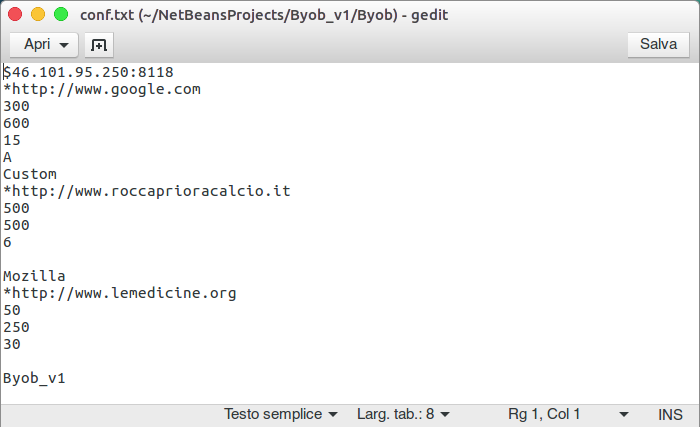
\includegraphics[width=0.7\linewidth]{imgs/conf}
\caption{File di configurazione}
\label{fig:conf}
\end{figure}

\begin{figure}[htp]
\centering
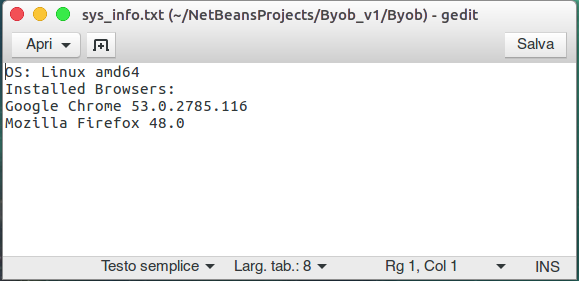
\includegraphics[width=0.7\linewidth]{imgs/sys_info}
\caption{Informazioni del Sistema}
\label{fig:sys_info}
\end{figure}

\begin{figure}[htp]
\centering
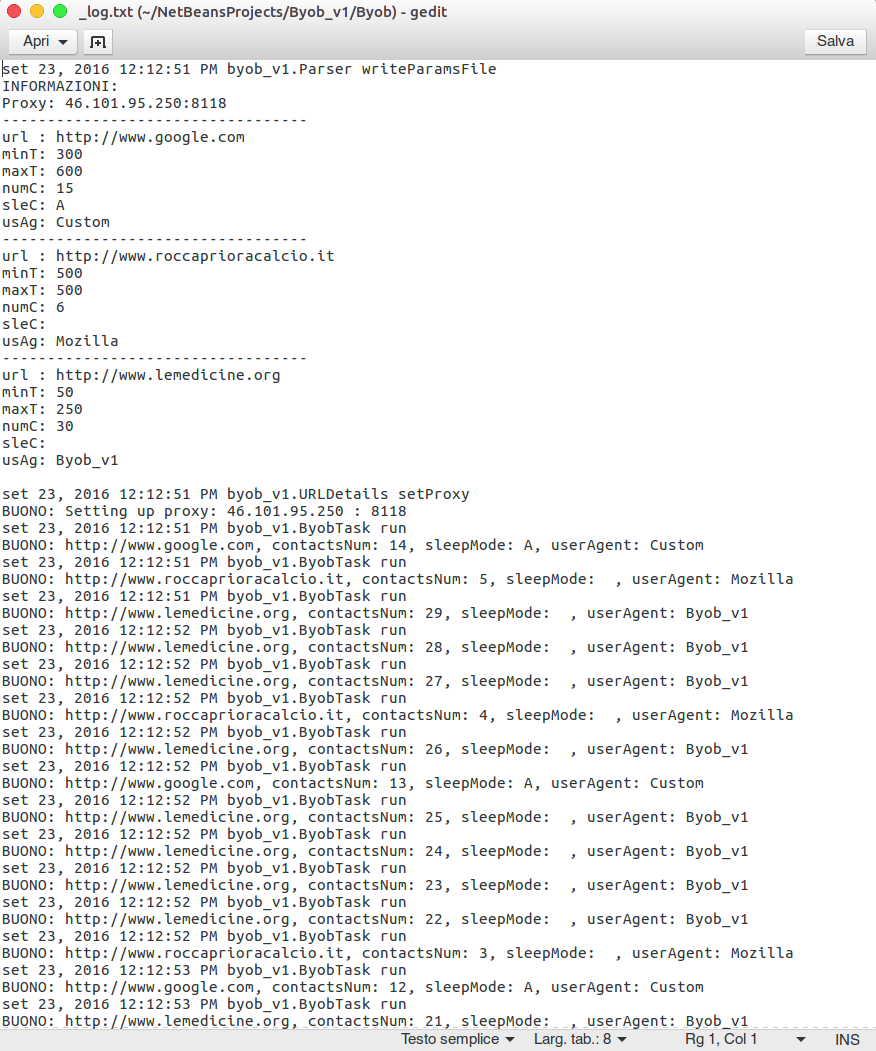
\includegraphics[width=0.7\linewidth]{imgs/log}
\caption{File di log}
\label{fig:log}
\end{figure}

\newpage
La verifica dei contatti avvenuti con le \textit{URL} specificate \`{e} stato facilitato dall'utilizzo di un software di monitoraggio grafico della rete chiamato \textit{EtherApe}\footnote{http://etherape.sourceforge.net/}

\vspace{0.5cm}
\begin{figure}[htp]
\centering
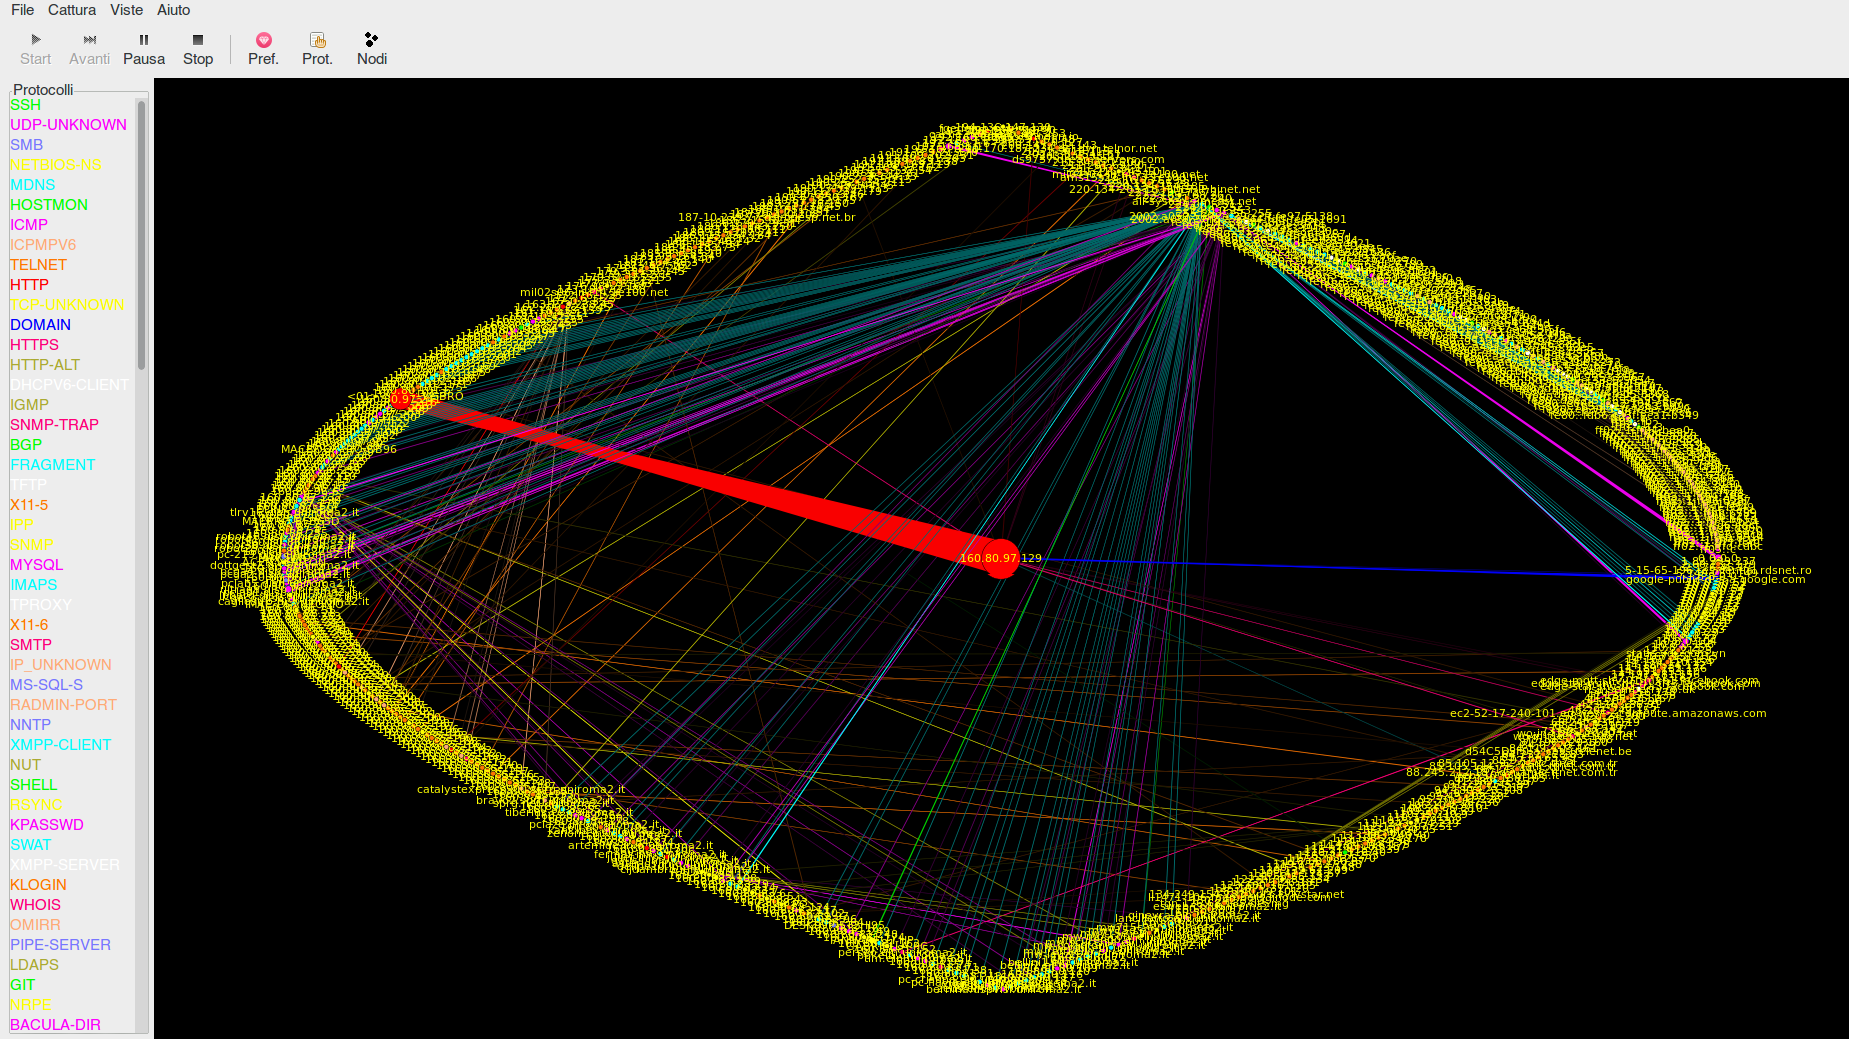
\includegraphics[width=1\linewidth]{imgs/etherape}
\caption{Graphical network monitor: etherApe}
\label{fig:etherape}
\end{figure}


\chapter{Installazione}

Il software non viene rilasciato con un \textit{Installer}, ma \`{e} possibile effettuarne l'esecuzione in maniera diretta:
\begin{itemize}
	\item in ambiente Windows, su cui \`{e} stato installato un \textit{Java Runtime Environment}, \`{e} sufficiente effettuare un doppio click sul file \textit{Byob\_v1.jar};
	
	\item in ambiente Unix, basta eseguire da terminale il comando
	\begin{lstlisting}
	java -jar Byob\_v1.jar
	\end{lstlisting}
\end{itemize}

All'inizio dell'esecuzione, verr\`{a} creata la cartella \textit{Byob} nella directory corrente, che conterr\`{a} i file \textit{\_log.txt} e \textit{sys\_info.txt}.
%\include{conclusioni}

%\begin{document}


\end{document}